%! Author = antonio
%! Date = 7/2/24

Logistic Regression is a discriminative classification model, directly evaluating the posterior probability \(C \mid X\).
In particular by determining that hyperplane which maximises the posterior probability.
Starting from the results obtained from the Tied Gaussian that provides log-likelihood ratios that are linear functions
of our data, where log-posterior probability ratio is:

\begin{equation}
    \log \frac{P(C=h_1 \mid X)}{P(C=h_0 \mid X)} = \log \frac{f_{X \mid C}(x \mid h_1)}{f_{X \mid C}(x \mid h_0)} + \log \frac{\pi}{1-\pi} = \omega^T x + b
    \label{eq:logisticRegression}
\end{equation}

where prior information has been absorbed in the bias term \(b\) of the \autoref{eq:logisticRegression}.
So from this point we can define the score function as:

\begin{equation}
    s(x) = \omega^T x + b = 0
    \label{eq:scoreFunctionLR}
\end{equation}

where it is positive for samples of class \(h_1\) and negative for samples of class \(h_0\).
Given \(\omega\) and \(b\) we can compute the posterior class probability as:

\begin{equation}
    P(C=h_1 \mid x, \omega, b) = \sigma(\omega^T x + b) = \sigma(s(x))
    \label{eq:posteriorClassProbabilityLR}
\end{equation}
where \(\sigma\) is sigmoid function defined as:

\begin{equation}
    \sigma(x) = \frac{1}{1 + e^{-x}}
\end{equation}

This approach assumes that the decision rules will be hyperplanes orthogonal to vector w.

\subsubsection{Binary Logistic Regression}
\textbf{Binary Logistic Regression Not Prior-Weighted}\par
The objective is to minimise the loss function \(J(\omega,b)\), but to this is introduced what is a penalty term,
so the new function becomes:

\begin{equation}
    J(\omega,b) = \frac{\lambda}{2}\left\|w \right\|^2 + \frac{1}{n} \sum_{i=1}^{n} \log (1+e^{-z_i(\omega^T x_i + b)}), \quad
    z_i = \begin{cases}
              1 & \text{if } c_i = 1 \\
              -1 & \text{if } c_i = 0
    \end{cases}
    \label{eq:minimiseFunctionLR}
\end{equation}

where \(\lambda\) of \autoref{eq:minimiseFunctionLR} is the regularization term, this term has been introduced to make problem
solvable in case of linearly separable classes.

\begin{figure}[h!]
    \centering
    \begin{subfigure}[b]{0.40\linewidth}
        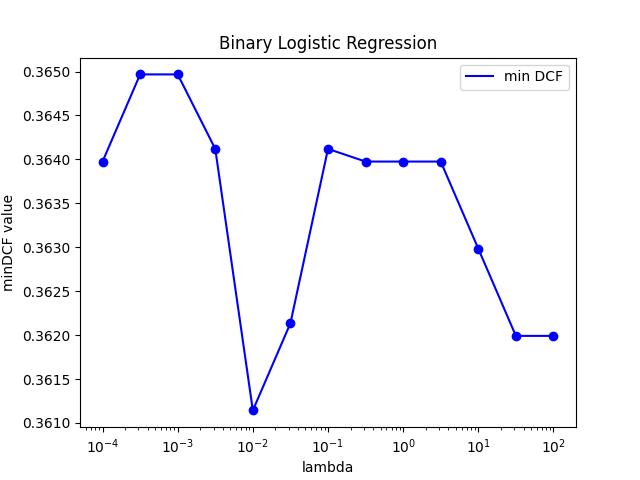
\includegraphics[width=\linewidth]{Lab/08. Lab 08/Images/01. BLR - minDCF}
        \label{fig:BLRminDCF}
    \end{subfigure}
    \begin{subfigure}[b]{0.40\linewidth}
        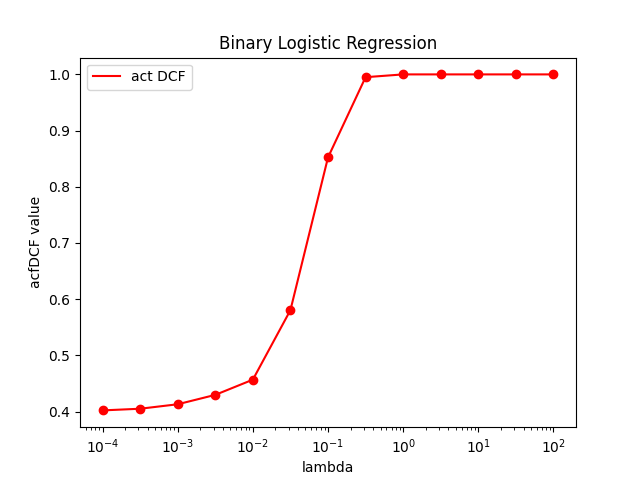
\includegraphics[width=\linewidth]{Lab/08. Lab 08/Images/02. BLR - actDCF}
        \label{fig:BLRactDCF}
    \end{subfigure}
    \begin{subfigure}[b]{0.40\linewidth}
        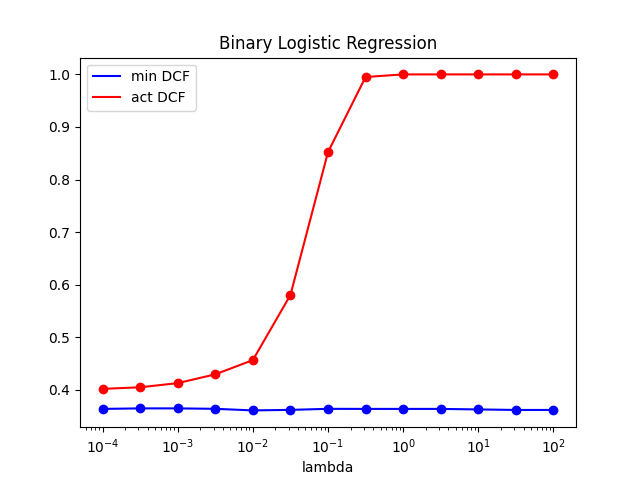
\includegraphics[width=\linewidth]{Lab/08. Lab 08/Images/03. BLR - min And actDCF}
        \label{fig:BLRminAndactDCF}
    \end{subfigure}
    \begin{subfigure}[b]{0.40\linewidth}
        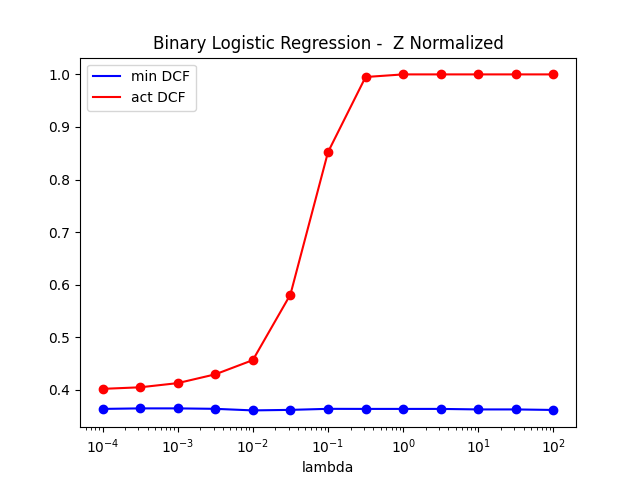
\includegraphics[width=\linewidth]{Lab/08. Lab 08/Images/04. BLR - minAnd actDCF - ZNormalized}
        \label{fig:BLRminAndactDCFZNorm}
    \end{subfigure}
    \caption{Binary Logistic Regression not Prior-Weighted}
    \label{fig:BLR}
\end{figure}

\begin{figure}[h!]
    \centering
    \begin{subfigure}[b]{0.40\linewidth}
        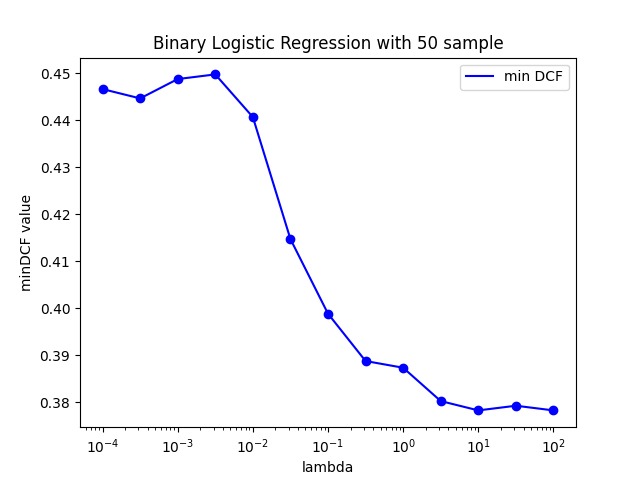
\includegraphics[width=\linewidth]{Lab/08. Lab 08/Images/05. BLR - minDCF 50 Samples}
        \label{fig:BLR50SminDCF}
    \end{subfigure}
    \begin{subfigure}[b]{0.40\linewidth}
        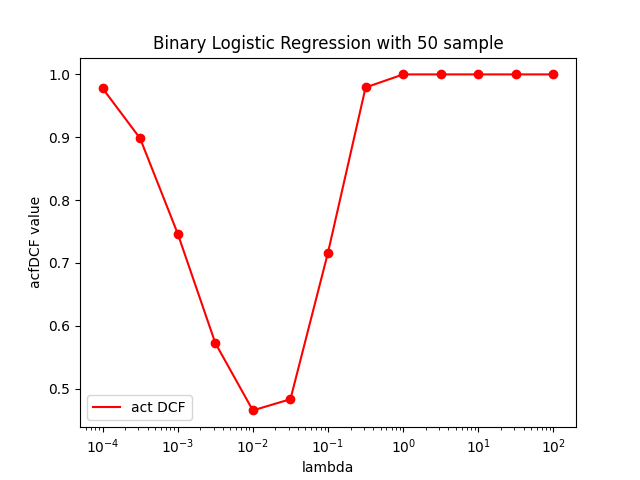
\includegraphics[width=\linewidth]{Lab/08. Lab 08/Images/06. BLR - actDCF 50 Samples}
        \label{fig:BLR50SactDCF}
    \end{subfigure}
    \begin{subfigure}[b]{0.40\linewidth}
        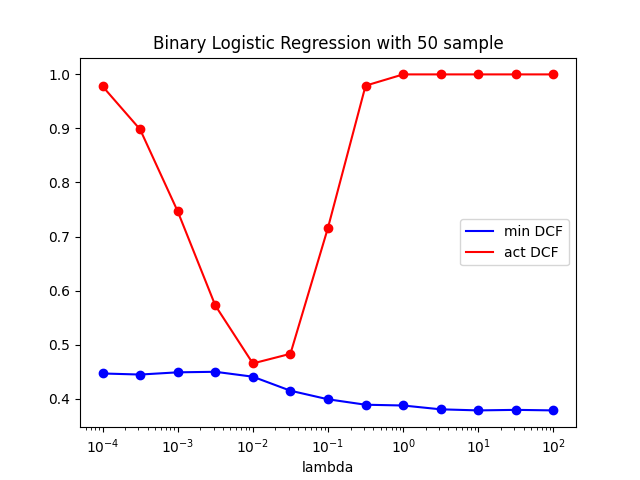
\includegraphics[width=\linewidth]{Lab/08. Lab 08/Images/07. BLR - minAndactDCF 50 Samples}
        \label{fig:BLR50SminAndactDCF}
    \end{subfigure}
    \begin{subfigure}[b]{0.40\linewidth}
        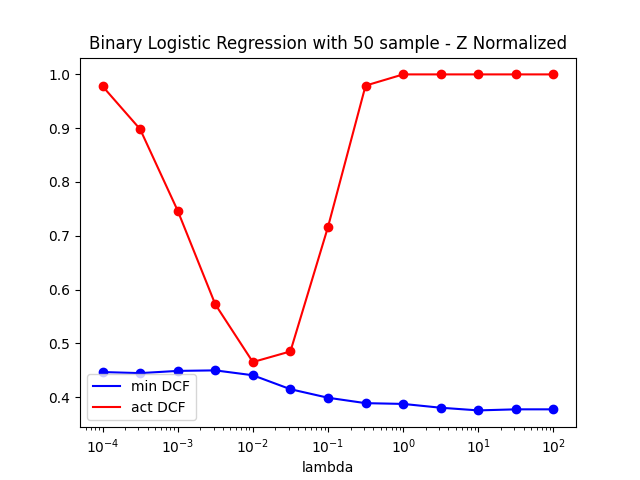
\includegraphics[width=\linewidth]{Lab/08. Lab 08/Images/08. BLR - minAndactDCF 50 Samples - ZNormalized}
        \label{fig:minAndactDCFZNorm}
    \end{subfigure}
    \caption{Binary Logistic Regression not Prior-Weighted with 50 Samples}
    \label{fig:BLR50Samples}
\end{figure}

In this model \(\pi_T = 0.1\) is used.
In \autoref{tab:minDCFactDCFBLRNPW}, it can be seen how the values of minDCF and actDCF vary when \(\lambda\) changes,
Z-normalization is applied or not and if the whole training set or a portion was used.
It can be deduced from the values obtained that the application of z-normalisation brings no advantage.
On the other hand, by using only 50 samples, it can see that using a limited number of samples can significantly
influence the model and could lead to misleading results that are not representative of the entire sample.
Consequently, as many samples as possible should be used for training to obtain a more accurate model.
\autoref{fig:BLR} and \autoref{fig:BLR50Samples} give a graphic representation of how minDCF and actDCF vary with \(\lambda\)

\begin{table}[h!]
    \centering
    \begin{tabular}{>{\centering\arraybackslash}p{2cm} >{\centering\arraybackslash}p{2cm} >{\centering\arraybackslash}p{2cm} >{\centering\arraybackslash}p{2cm}>{\centering\arraybackslash}p{2cm}}
        \toprule
        \multicolumn{5}{c}{\textbf{Binary Logistic Regression Not Prior-Weighted}} \\
        \midrule
        \multirow{2}{*}{\centering \textbf{\(\lambda\)}} & \multicolumn{2}{c}{\textbf{minDCF}} & \multicolumn{2}{c}{\textbf{actDCF}} \\
        \cmidrule(lr){2-5}
        & \textbf{no z-norm} & \textbf{z-norm} & \textbf{no z-norm} & \textbf{z-norm} \\
        \midrule
        \(10^{-4}\) & 0.3640             & 0.3640          & 0.4021             & 0.4021          \\
        \(10^{-3}\) & 0.3650             & 0.3650          & 0.4130             & 0.4130          \\
        \(10^{-2}\) & 0.3611             & 0.3611          & 0.4568             & 0.4568          \\
        \(10^{-1}\) & 0.3641             & 0.3641          & 0.8522             & 0.8522          \\
        \midrule
        \midrule
        \multicolumn{5}{c}{\textbf{Binary Logistic Regression Not Prior-Weighted (50 Samples)}} \\
        \midrule
        \multirow{2}{*}{\centering \textbf{\(\lambda\)}} & \multicolumn{2}{c}{\textbf{minDCF}} & \multicolumn{2}{c}{\textbf{actDCF}} \\
        \cmidrule(lr){2-5}
        & \textbf{no z-norm} & \textbf{z-norm} & \textbf{no z-norm} & \textbf{z-norm} \\
        \midrule
        \(10^{-4}\) & 0.4466             & 0.4466          & 0.9780             & 0.9780          \\
        \(10^{-3}\) & 0.4487             & 0.4487          & 0.7466             & 0.7466          \\
        \(10^{-2}\) & 0.4407             & 0.4407          & 0.4652             & 0.4652          \\
        \(10^{-1}\) & 0.3988             & 0.3988          & 0.7164             & 0.7164          \\
        \bottomrule
    \end{tabular}
    \captionsetup{justification=justified,singlelinecheck=false,format=hang}
    \caption{Show minDCF and actDCF for Binary Logistic Regression Not Prior-Weighted model}
    \label{tab:minDCFactDCFBLRNPW}
\end{table}

\newpage
\textbf{Binary Logistic Regression Prior-Weighted}\par
Another possible Logistic Regression approach is that Prior-Weighted; it allows to simulate different priors for class 1.
Therefore, the objective function becomes:

\begin{equation}
    J(\omega,b) = \frac{\lambda}{2}\left\|w \right\|^2 + \sum_{i=1}^{n} \xi_i\log (1+e^{-z_i(\omega^T x_i + b)}),\quad
    \xi_i = \begin{cases}
                \frac{\pi_t}{n_T} & \text{if } z_i = +1 (c_i = 1) \\
                \frac{1 - \pi_T}{n_F} & \text{if } z_i = -1 (c_i = 0) \\
    \end{cases}
    \label{eq:minimiseFunctionLRPW}
\end{equation}

Now it is possible analyze the results obtained from the Prior-Weighted model with \(\pi_T = 0.1\).

\begin{figure}[h!]
    \centering
    \begin{subfigure}[b]{0.30\linewidth}
        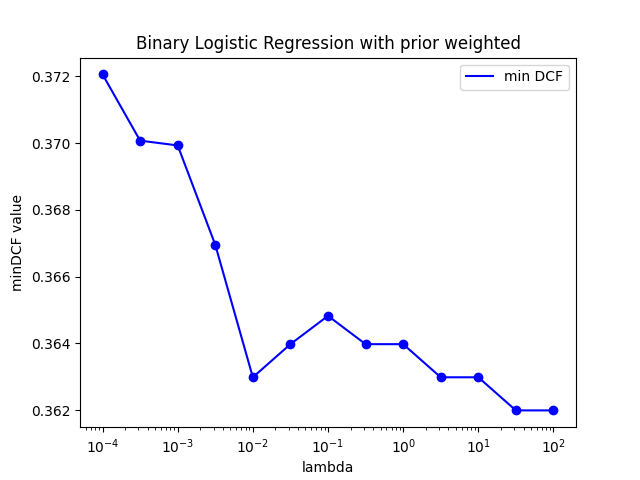
\includegraphics[width=\linewidth]{Lab/08. Lab 08/Images/09. PW - minDCF}
        \label{fig:PWminDCF}
    \end{subfigure}
    \begin{subfigure}[b]{0.30\linewidth}
        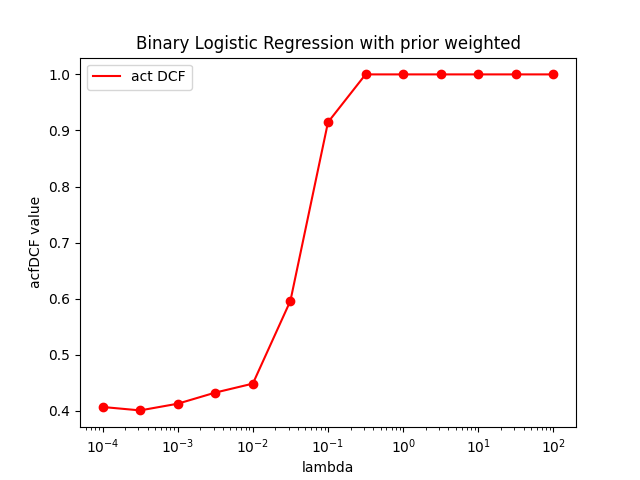
\includegraphics[width=\linewidth]{Lab/08. Lab 08/Images/10. PW - actDCF}
        \label{fig:PWactDCF}
    \end{subfigure}
    \begin{subfigure}[b]{0.30\linewidth}
        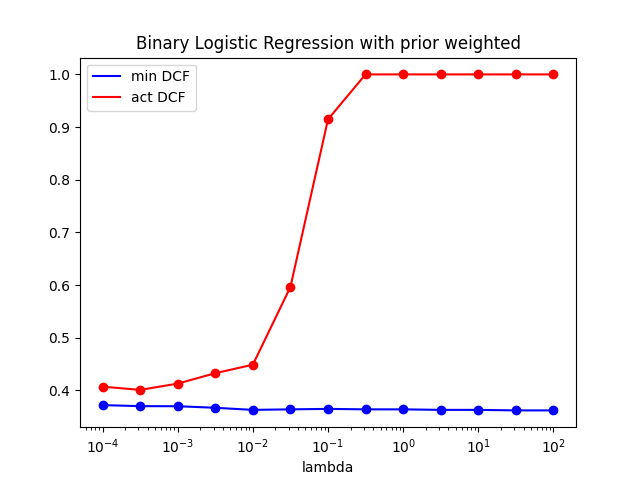
\includegraphics[width=\linewidth]{Lab/08. Lab 08/Images/11. PW - minAndActDCF}
        \label{fig:PWminAndactDCF}
    \end{subfigure}
    \caption{Binary Logistic Regression Prior-Weighted}
    \label{fig:PW}
\end{figure}

\begin{table}[h!]
    \centering
    \begin{tabular}{>{\centering\arraybackslash}p{2cm} >{\centering\arraybackslash}p{2cm} >{\centering\arraybackslash}p{2cm}}
        \toprule
        \multicolumn{3}{c}{\textbf{Binary Logistic Regression Prior-Weighted }} \\
        \midrule
        \multicolumn{3}{c}{\(\pi_T = 0.1 \)} \\
        \midrule
        \textbf{\(\lambda\)} & \textbf{minDCF} & \textbf{actDCF} \\
        \midrule
        \(10^{-4}\)          & 0.3721          & 0.4071          \\
        \(10^{-3}\)          & 0.3699          & 0.4129          \\
        \(10^{-2}\)          & 0.3630          & 0.4487          \\
        \(10^{-1}\)          & 0.3648          & 0.9147          \\
        \bottomrule
    \end{tabular}
    \captionsetup{justification=justified,singlelinecheck=false,format=hang}
    \caption{Show minDCF and actDCF for Binary Logistic Regression Prior-Weighted}
    \label{tab:minDCFactDCFPW}
\end{table}

The role of the prior is to weight the samples during model training.
In particular, samples in the higher priority class receive a higher weight than those in the lower priority class.
This can be useful if the dataset is unbalanced, the choice of the prior must be made at the beginning and this choice
can affect the model a lot, in fact we may even have a worsening of the model. \\
Comparing the results obtained in \autoref{tab:minDCFactDCFBLRNPW} and \autoref{tab:minDCFactDCFPW},
there isn't noticeable change in the outcomes on minDCF and actDCF this means that our dataset is not unbalanced.
The interesting value to observe is the value of actDCF when \(\lambda= 10^-1\).\\

\textbf{Binary Logistic Regression with Pre-processing (PCA)}\par
In this case, PCA can be applied as pre-processing, and by looking at the values in \autoref{tab:minDCFactDCFBLPCA},
it can be seen that it does not result much improvement of the system.

\begin{figure}[h!]
    \centering
    \begin{subfigure}[b]{0.30\linewidth}
        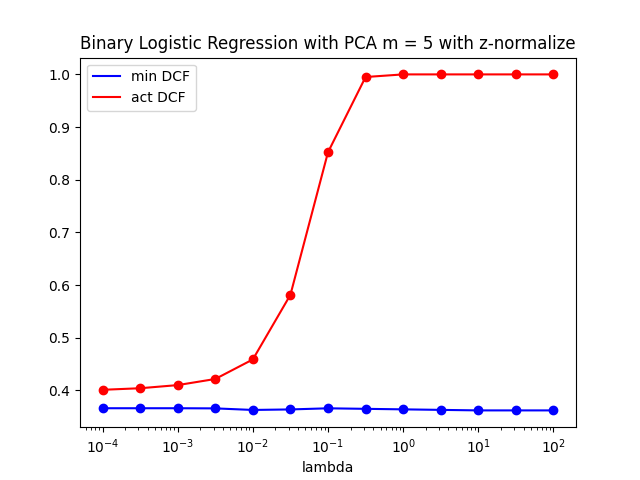
\includegraphics[width=\linewidth]{Lab/08. Lab 08/Images/12. BLR - PCA m=5 Z-norm}
        \label{fig:BLRPCAm5ZNorm}
    \end{subfigure}
    \begin{subfigure}[b]{0.30\linewidth}
        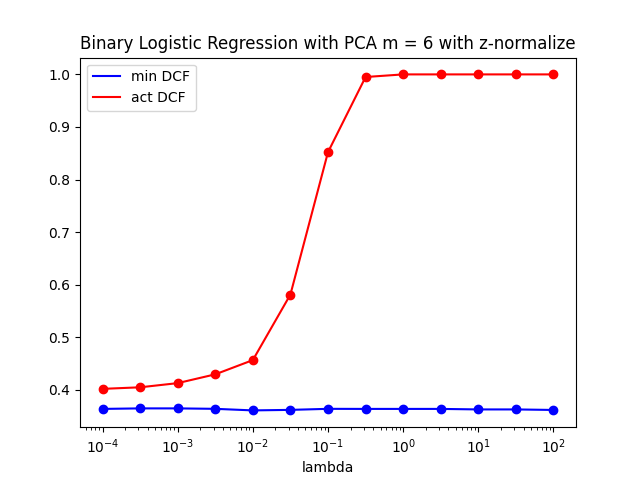
\includegraphics[width=\linewidth]{Lab/08. Lab 08/Images/13. BLR - PCA m=6 Z-norm}
        \label{fig:BLRPCAm6ZNorm}
    \end{subfigure}
    \caption{Binary Logistic Regression applying PCA and z-normalization}
    \label{fig:BLRPCA}
\end{figure}

\begin{table}[h!]
    \centering
    \begin{tabular}{>{\centering\arraybackslash}p{2cm} >{\centering\arraybackslash}p{2cm} >{\centering\arraybackslash}p{2cm}>{\centering\arraybackslash}p{2cm}>{\centering\arraybackslash}p{2cm}}
        \toprule
        \multicolumn{5}{c}{\textbf{Binary Logistic Regression with PCA }} \\
        \midrule
        \multirow{2}{*}{\centering \textbf{\(\lambda\)}} & \multicolumn{2}{c}{\textbf{minDCF}} & \multicolumn{2}{c}{\textbf{actDCF}} \\
        \cmidrule(lr){2-5}
        & \textbf{no z-norm} & \textbf{z-norm} & \textbf{no z-norm} & \textbf{z-norm} \\
        \midrule
        \multicolumn{5}{c}{\textbf{\(m=5\)}} \\
        \midrule
        \(10^{-4}\) & 0.3661             & 0.3661          & 0.4011             & 0.4011          \\
        \(10^{-3}\) & 0.3661             & 0.3661          & 0.4100             & 0.4100          \\
        \(10^{-2}\) & 0.3618             & 0.3628          & 0.4578             & 0.4588          \\
        \(10^{-1}\) & 0.3660             & 0.3660          & 0.8502             & 0.8522          \\
        \midrule
        \multicolumn{5}{c}{\textbf{\(m=6\)}} \\
        \midrule
        \(10^{-4}\) & 0.3640             & 0.3640          & 0.4021             & 0.4021          \\
        \(10^{-3}\) & 0.3650             & 0.3650          & 0.4130             & 0.4130          \\
        \(10^{-2}\) & 0.3611             & 0.3611          & 0.4568             & 0.4568          \\
        \(10^{-1}\) & 0.3641             & 0.3641          & 0.8522             & 0.8522          \\
        \bottomrule
    \end{tabular}
    \captionsetup{justification=justified,singlelinecheck=false,format=hang}
    \caption{Show minDCF and actDCF for Binary Logistic Regression applying PCA and with adn withoud z-normalization}
    \label{tab:minDCFactDCFBLPCA}
\end{table}

\subsubsection{Quadratic Logistic Regression}
In this step we can analyze training on a Quadratic Logistic Regression model by performing features expansion, so it's possible write log-likelihood ratio as:
\begin{equation}
    \log{\frac{P(C=h_1|x)}{P(C=h_0|x)}}=x^TAx+b^Tx+c=s(\textbf{x},\textbf{A},\textbf{b},\textbf{c})
\end{equation}
This expression is quadratic in x but it's linear in A and b.
We could rewrite it to obtain a decision function that is linear for the expanded features space but quadratic in original features space.\\
We can write features expansion as:
\begin{equation}
    \Phi(x)=
    \begin{bmatrix}
        vec(xx^T) \\
        x
    \end{bmatrix},
    \;\;
    w=
    \begin{bmatrix}
        vec(A) \\
        b
    \end{bmatrix}
\end{equation}
where vec(X) is the operator that stacks the columns of X into a single column vector. In this way we can write the posterio log-likelihood as:
\begin{equation}
    s(x,w,c)=s^T\phi(x)+c
\end{equation}

%Tabella
%
%In conclusion, the results obtained from the Quadratic Logistic Regression model show that